\documentclass{beamer}
\usepackage[utf8]{inputenc}
\usepackage{amsmath}
\usepackage{amsfonts}
\usepackage{graphicx}
\usepackage{subcaption}
\setbeameroption{show notes}
\usepackage[sorting=none,backend=bibtex,style=numeric]{biblatex}
\addbibresource{../bibliography/aci-bibliography.bib}
\renewcommand*{\bibfont}{\scriptsize}

\useoutertheme{tree}

\title{Animation character identification from color images}
\author{Alexis Vallet, Yuki Nakagawa, Hiroyasu Sakamoto}
\institute{Kyushu University, University of Technology of Belfort-Montbéliard}

\begin{document}
\frame{\titlepage}

\section{Animation character identification}

\begin{frame}
\begin{itemize}
\item (Semi) supervised classification of animation character images.
\item Dealing with variations in character posture, occlusion, drawing style, exaggerations.
\item Application domain: web artist communities such as Pixiv, deviantArt.
\end{itemize}

\begin{figure}[htb!]
\centering
\begin{subfigure}{.3\textwidth}

\includegraphics[width=\textwidth]{../images/miku_e.png}
\end{subfigure}
\begin{subfigure}{.3\textwidth}

\includegraphics[width=\textwidth]{../images/miku_c.png}
\end{subfigure}
\begin{subfigure}{.3\textwidth}

\includegraphics[width=\textwidth]{../images/miku_d.png}
\end{subfigure}
\caption{Images illustrating variations for a single character.}
\label{fig:animationImagesVariations}
\end{figure}

\end{frame}

\begin{frame}
\begin{itemize}
\item Preprocessing: removing outlines, switching color space.
\item Segmentation to isolate parts of interest - hair, clothes, face...
\item Classification by comparing segmentation against training set.
\end{itemize}

\begin{figure}[htb!]
\centerline{
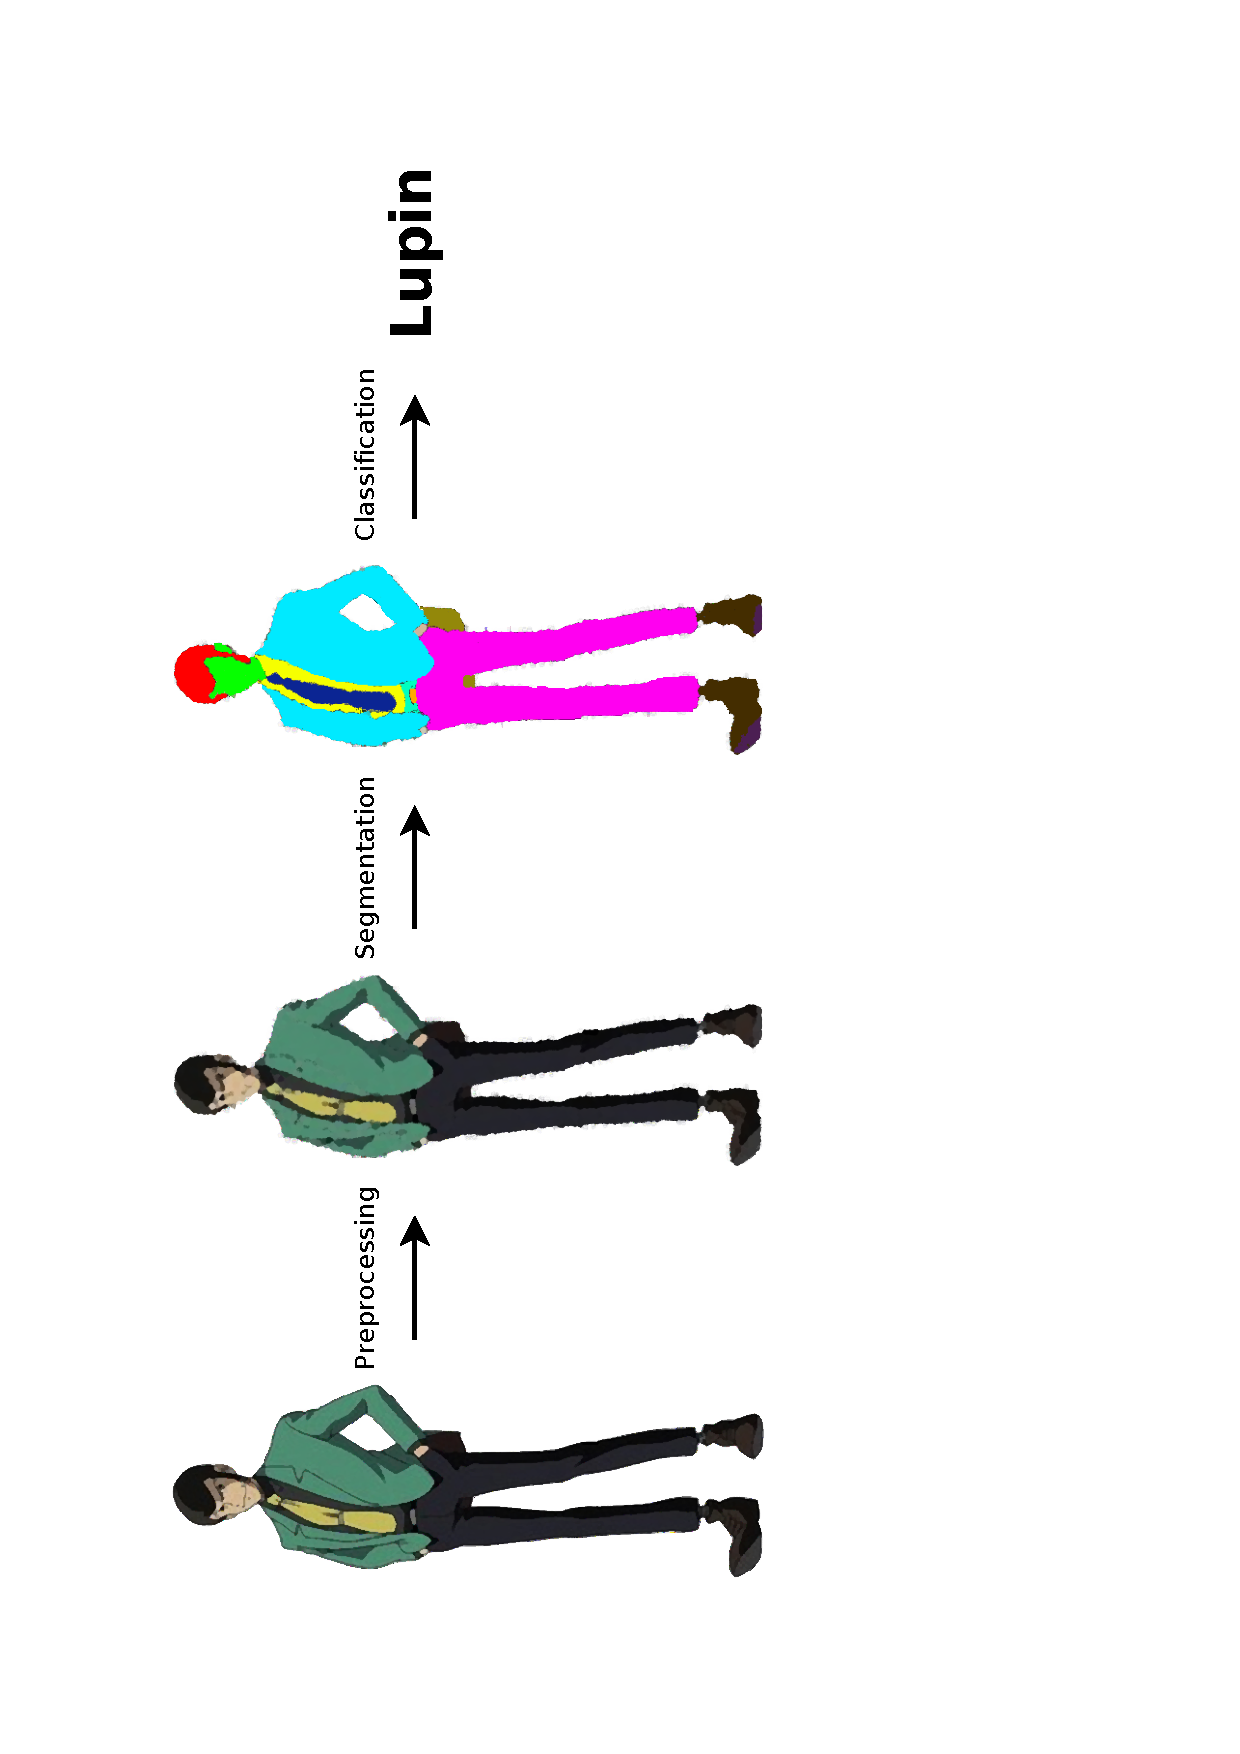
\includegraphics[height=\textwidth,angle=270,clip=true,trim=2cm 0 6cm 0]{../images/visionSystemDiagram.pdf}
}
\caption{Diagram depicting how preprocessing, segmentation and classification interact.}
\end{figure}

\end{frame}

\section{Segmentation by Felzenszwalb's method}

\begin{frame}
\frametitle{Felzenszwalb' segmentation \cite{felzenszwalb2004efficient}}

\begin{itemize}
\item Graph method based on Kruskal's algorithm.
\item Efficient: $O(n\log(n))$ time with $4$-connected neighborhood.
\item Accurate: neither too "coarse" nor too "fine".
\item But depends on a scale parameter $k$ which controls the size of segments.
\end{itemize}

\begin{figure}[htb!]
\centering
\begin{subfigure}{.3\textwidth}

\includegraphics[width=\textwidth]{../images/rufy_d.png}
\caption{Original image}
\end{subfigure}
\begin{subfigure}{.3\textwidth}

\includegraphics[width=\textwidth]{../images/luffyK100.png}
\caption{$k = 100$.}
\label{fig:smallKSegmentation}
\end{subfigure}
\begin{subfigure}{.3\textwidth}

\includegraphics[width=\textwidth]{../images/luffyK1000.png}
\caption{$k = 1000$.}
\label{fig:largeKSegmentation}
\end{subfigure}
\end{figure}

\end{frame}

\begin{frame}
\begin{itemize}
\item Post processing by merging segments with close hue.
\item Allows varying segment sizes and non connected segments.
\end{itemize}

\begin{figure}[htb!]
\centering
\begin{subfigure}{0.3\textwidth}

\includegraphics[width=\textwidth]{../images/miku_a.png}
\caption{Original image.}
\end{subfigure}
\begin{subfigure}{0.3\textwidth}
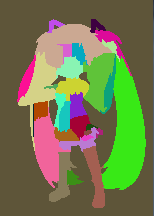
\includegraphics[width=\textwidth]{../images/miku_seg_initial.png}
\caption{Before merging.}
\end{subfigure}
\begin{subfigure}{0.3\textwidth}
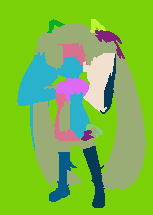
\includegraphics[width=\textwidth]{../images/miku_seg_fused.png}
\caption{After merging.}
\end{subfigure}
\end{figure}
\end{frame}

\section{Classification by spectral method}

\begin{frame}
\frametitle{Spectral classification method}
\begin{itemize}
\item For segmentation $S$ consider features $(f_i : S \rightarrow \mathbb{R}^q_i)_{1 \leq i \leq m}$. (average color, gravity center, size...)
\item For each feature $f_i$, compute $K$-nearest neighbor graph $G_i$ on $S$ with weights $w(u,v) = e^{-\frac{||f_i(S_u) - f_i(S_v)||^2}{\sigma_i^2}}$ and Laplacian $L_i$.
\end{itemize}

\begin{figure}[htb!]
\centering
\begin{subfigure}{0.3\textwidth}
\centering
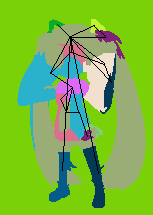
\includegraphics[width=0.7\textwidth]{../images/miku_seg_graph.png}
\caption{Example of graph on $S$.}
\end{subfigure}
\begin{subfigure}{0.65\textwidth}
\resizebox{\hsize}{!}{
$L_i(u,v) = \begin{cases}
\sum_{u'\text{ adjacent to }u} w(u,u') & \text{if } u = v\\
-w(u,v) & \text{if $u$ and $v$ are adjacent}\\
0 & \text{otherwise}
\end{cases}$
}
\caption{Laplacian matrix definition.}
\end{subfigure}
\end{figure}
\end{frame}

\begin{frame}
\begin{itemize}
\item Only use the eigenvectors from the $k$ smallest nonzero eigenvalues of $L_i$.
\item Use method from Wilson, Hancock, Luo to create pattern vectors $B_i$ from these eigenvectors \cite{wilson2005pattern}.
\item Concatenate into feature vector $B = (B_1^T ... B_m^T)$, classify using SVM.
\end{itemize}
\end{frame}

\begin{frame}
\frametitle{Results and analysis}
\begin{itemize}
\item Low recognition rate (close to random).
\item Graphs do not encode enough information about individual segments.
\item Deals poorly with different number of segments.
\end{itemize}
\end{frame}

\section{Classification by segment matching}

\begin{frame}
\frametitle{Segment matching classification}
\begin{itemize}
\item Consider $3$ features for each segment: average $L^*a^*b^*$ color, gravity center, and area.
\item Measure similarity between segments using a fuzzy system.
\item Find a one to one relation between similar segments of $2$ images.
\end{itemize}

\begin{figure}
\centering
\begin{subfigure}{0.24\textwidth}

\includegraphics[width=\textwidth]{../images/rufy_d.png}
\end{subfigure}
\begin{subfigure}{0.24\textwidth}
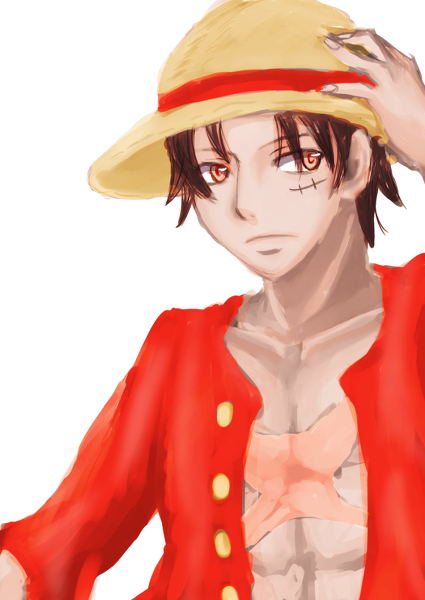
\includegraphics[width=\textwidth]{../images/rufy_original2.png}
\end{subfigure}
\begin{subfigure}{0.24\textwidth}
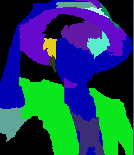
\includegraphics[width=\textwidth]{../images/luffy_match1.png}x
\end{subfigure}
\begin{subfigure}{0.24\textwidth}
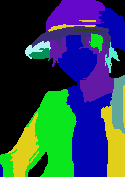
\includegraphics[width=\textwidth]{../images/luffy_match2.png}
\end{subfigure}
\caption{Original images (left) and corresponding relation (right). Segments with the same color are matched together.}
\end{figure}

\end{frame}

\begin{frame}
\begin{itemize}
\item Measure overall similarity $sim(S,T)$ between segmentation $S$ and $T$ by sum of matching segments similarity weighted by segment areas.
\item Classify by nearest neighbor.
\end{itemize}

\begin{figure}
\centering
\begin{subfigure}{0.3\textwidth}
\centering
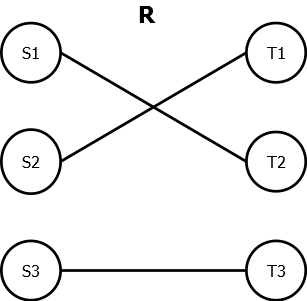
\includegraphics[width=\textwidth]{../images/relation.png}
\end{subfigure}
\begin{subfigure}{0.5\textwidth}
\centering
\[ \quad sim(S,T) = \sum_{(S_i,T_j) \in R}(|S_i| + |T_j|)s_{ij}\]
\end{subfigure}
\end{figure}

Where $s_{ij}$ denotes the similarity between segments $S_i$ and $T_j$ by the fuzzy system.

\end{frame}

\begin{frame}
\frametitle{Results and analysis}
\begin{itemize}
\item $59\%$ recognition rate for dataset with 12 characters and 15 images per characters.
\item Recognition rate scales well with size of dataset.
\item Has trouble with characters sharing similar color palette.
\end{itemize}

\begin{figure}[htb!]
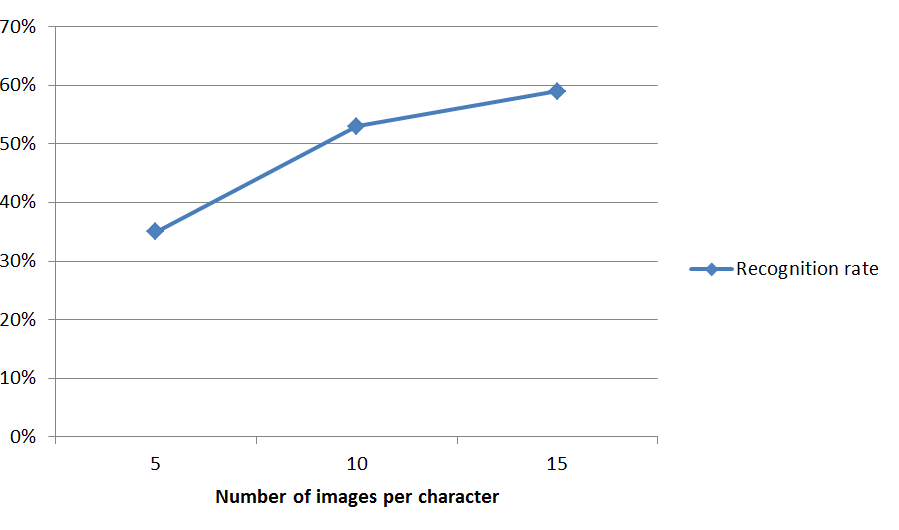
\includegraphics[width=0.8\textwidth]{../images/recognitionRate.png}
\end{figure}

\end{frame}

\begin{frame}
Possible extensions:

\begin{itemize}
\item Color palette issues: determining a (possibly non-linear, or high-dimensional) color space ideally separating training data, with some (semi) supervised embedding method  \cite{urahama2007semi} ?
\item Background extraction: detecting important character features (face, hair, clothes) using method inspired by the face detection algorithm from Viola and Jones \cite{viola2004robust} ?
\item Also using segmentation graph, as in works from Bach and Harchaoui \cite{harchaoui2007image} ?
\end{itemize}
\end{frame}

\section{References}
\begin{frame}
\frametitle{References}
\begin{small}
\printbibliography
\end{small}
\end{frame}

\end{document}